\section{Methodology}
\label{method}

% \begin{figure}
%     \centering
%     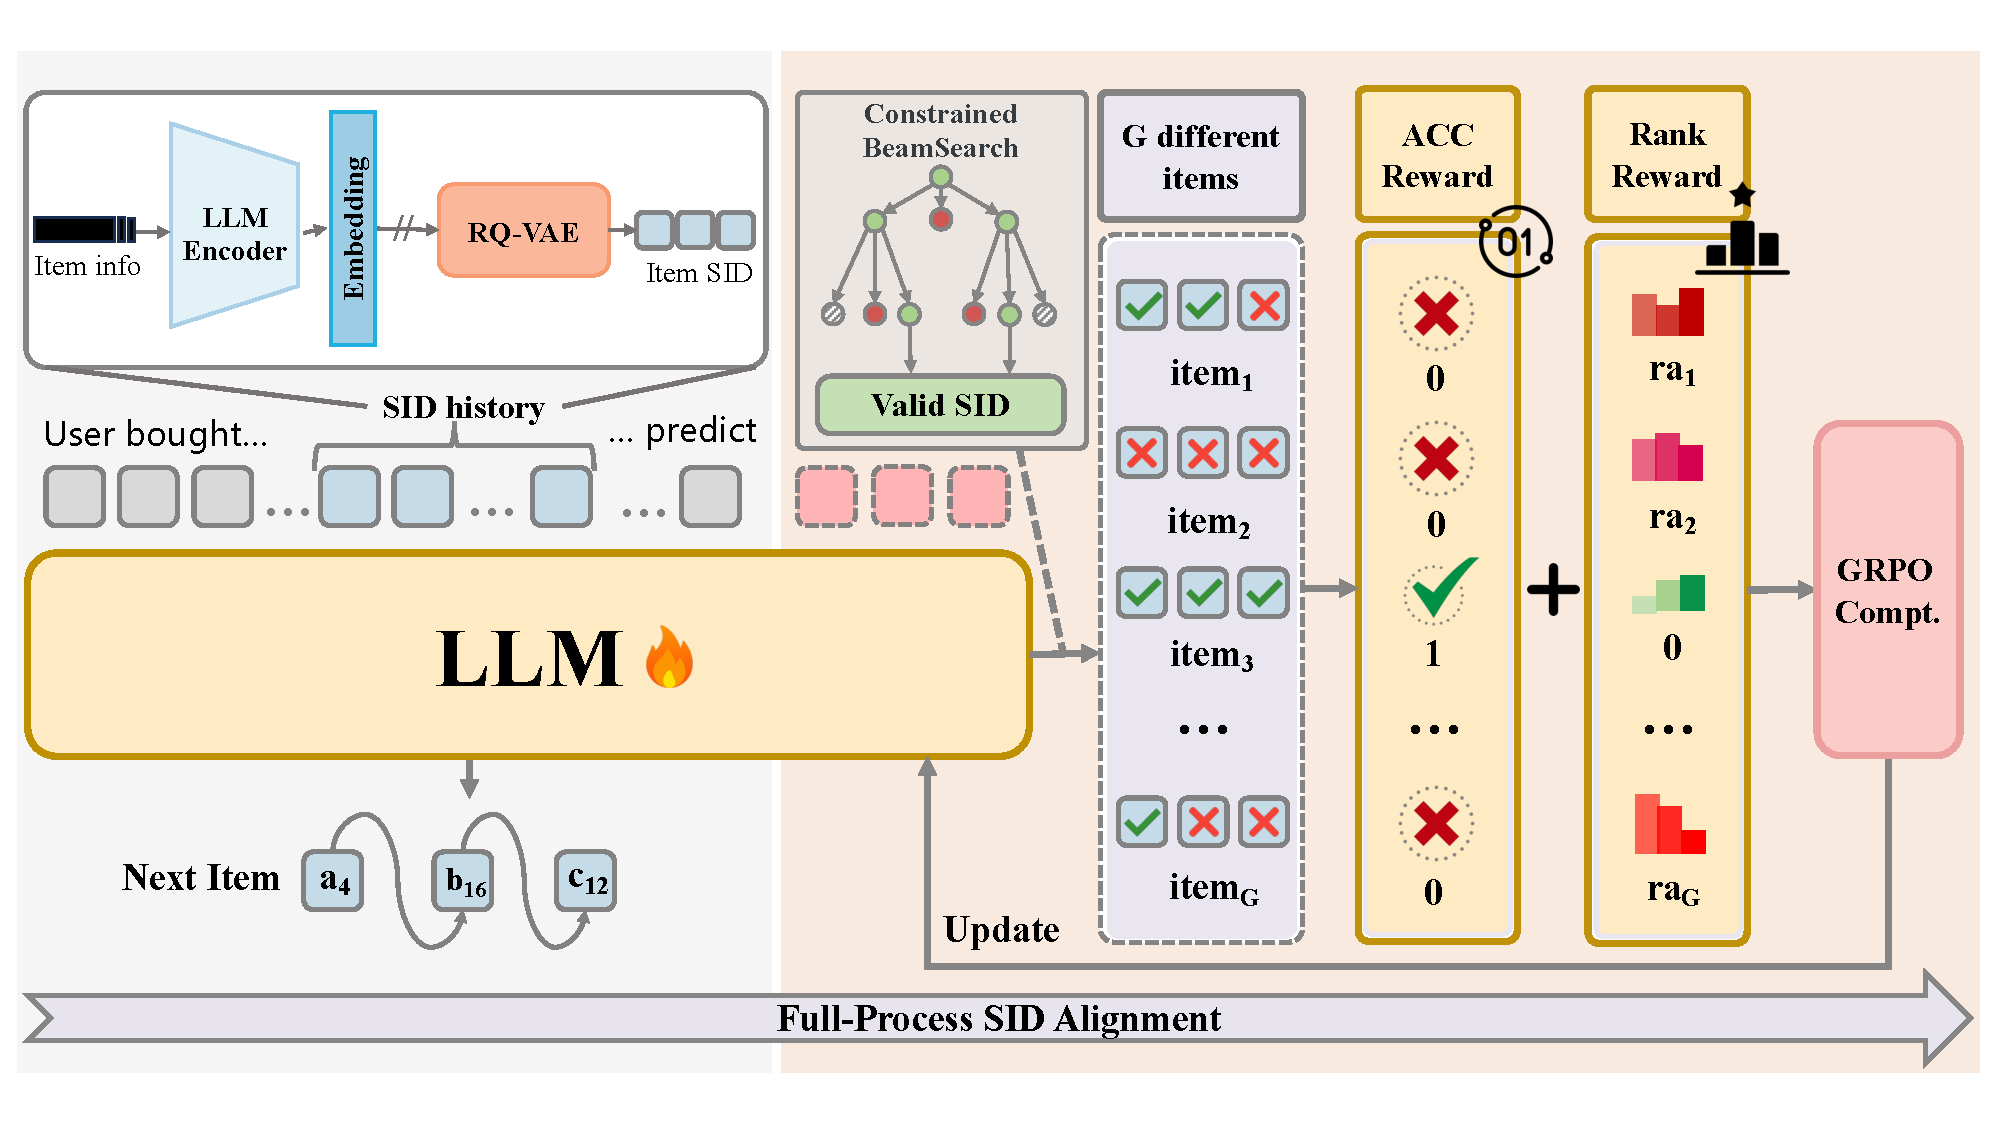
\includegraphics[width=0.85\textwidth]{figures/MiniOneRec_framework.pdf}
%     \vspace{-10pt}
%     \caption{MiniOneRec framework. RQ-VAE builds the item SID codebook. We then perform SFT to warm up the LLM and obtain an initial alignment. In RL, beam search with constrained decoding, thereby the model sequentially produces a ranked list of distinct, valid SIDs. GRPO updates the policy, and SID alignment is enforced end-to-end. This alignment objective is preserved throughout both the SFT and RL stages, fostering deeper semantic understanding.}
%     \label{fig:framework}
%     \vspace{-10pt}
% \end{figure}


To address the key shortcomings of the existing SFT-then-RL pipeline for generative recommendation, we propose \textbf{MiniOneRec}.  
The framework elevates the performance ceiling by aligning the LLM with the SID space throughout the entire training process and applying preference optimization in the RL stage, as illustrated in Figure \ref{fig:framework}.

\subsection{Full-Process SID Alignment}

As demonstrated in Section~\ref{llmmatter}, aligning world knowledge with item SIDs is beneficial for generative recommendation.  
Hence, instead of the paradigm that trains only on SIDs \citep{TIGER, OneRec, mtgr}, our LLM-based recommender explicitly strengthens the link between language understanding and collaborative semantics by injecting a set of alignment objectives:
\begin{itemize}[leftmargin=*]
    \item \textbf{Semantic Tasks.} 
    Given a chronologically ordered sequence of historical SIDs and an explicit task instruction, the LLM is asked to predict the SID of the next item the user is likely to interact with. 
    \item \textbf{Alignment Tasks.} % Bridging tasks that transfer knowledge between the semantic and textual spaces. 
It comprises a series of alignment tasks between the textual space and the SID space. Through these tasks, we encourage a bidirectional mapping that grounds SIDs in language and injects linguistic knowledge into SID representations.
\end{itemize}
Representative tasks from each category are jointly optimized throughout the entire SFT-then-RL pipeline, enabling the LLM to fully exploit its world knowledge, deepen its understanding of SIDs, and ultimately boost generative-recommendation performance. During the RL phase, we employ constrained decoding, limiting the output space to a precompiled dictionary that contains the SID of each item as well as its canonical title. This restriction ensures that the LLM can emit only legal identifiers, making it straightforward to compute a rule-based, verifiable reward signal. Detailed examples of the prompts are provided in the Appendix \ref{appendix:align_prompt}.

% \subsection{SID-Natigated Reinforcement Learning}
\subsection{Preference Optimization Reinforcement Learning}
% To fully exploit the fine-grained signals carried by SIDs, we introduce SID-Natigated Reinforcement Learning (SIN-RL).  
% SIN-RL comprises two complementary components—curriculum sampling and reward modeling.  
% By leveraging the codebook’s inherent coarse-to-fine hierarchy, SIN-RL steers the agent toward harder examples in a structured manner, thereby improving its capability in the challenging regions of the data distribution.
\tjf{Adapting RLVR to recommendation is not straightforward, as it raises two key challenges in sampling and reward design.
First, unlike open-ended language generation, the output space of recommendation is constrained to valid item SIDs. 
It is much narrower and makes repeated sampling from the same prompt prone to severe duplication, which in turn leads to low sampling efficiency. 
To mitigate this, we incorporate dynamic sampling \citep{DAPO} and constrained beam search to improve sampling efficiency and expose the model to more informative negative items.

On the other hand, while ranking ability is essential for recommendation, the rule-based reward assigns zero to all negatives, providing only coarse-grained feedback. 
This exposes a broader challenge: reward design in recommendation remains under-explored, yet holds significant potential for richer supervision. 
To move beyond binary correctness, we propose an auxiliary ranking reward that penalizes harder negatives with lower scores, and further investigate the potential of dense rewards such as semantic and collaborative signals.

\subsubsection{Sampling Strategy}
\label{subsection:sampling}
A key challenge in adapting RLVR to recommendation lies in the low sampling efficiency caused by the narrow item space: repeatedly sampling from the same prompt often yields duplicate items, reducing the diversity of sampled negatives. 
To quantify this, we define generation diversity as
\begin{align}
    \label{eq:diversity}
    \text{div}(\{e_k\}_{k=1}^G)=\frac{\text{uni}(\{e_k\}_{k=1}^G)}{G},
\end{align}
where $\text{uni}(\{e_k\}_{k=1}^G)$ counts the number of unique items among $G$ generations. 
Higher diversity exposes the model to richer negative signals and thus improves ranking supervision.
To enhance sampling efficiency, we explore two complementary strategies.
We first explore dynamic sampling, which over-generates candidates and then selects a subset that balances inclusion of the target item with maximizing negative diversity. 
However, this strategy requires generating substantially more samples, and its diversity also inevitably declines as training progresses. 
Motivated by these limitations, we ultimately adopt beam search as our sampling method. 
Beam search ensures that all sampled items are distinct, thereby improving efficiency and diversity. 
Following \citep{Decodingmatters}, we remove length normalization to avoid amplification bias.
%, with additional details reported in Appendix~\ref{Appendix:ConsBeamSearch}.}


\subsubsection{Reward Design}
\label{method:reward}
Recommendation quality is usually measured by ranking metrics like NDCG, highlighting the importance of fine-grained ranking ability. 
However, the rule-based reward in GRPO only distinguishes the target item from all others, assigning $1$ to the positive and $0$ to every negative.
This implicitly assumes that all negatives contribute equally during optimization and only injects coarse-grained ranking information into LLMs.
% To further corroborate our analysis, we provide a gradient study of GRPO in Appendix \ref{Appendix:gradient}.

% assigning larger gradients to hard negatives 
Prior works have shown that emphasizing hard negatives improves the discriminative ability of recommendation models \citep{SGL, sdpo}.
Motivated by this insight, we introduce a ranking reward penalizing harder negatives more heavily. 
Specifically, for a generated negative item $e_k$, we compute its generation rank $\rho_k$ and assign a lower reward to negatives with higher-probability:
\begin{align}
    \hat{R}_\text{rank}(e_k, e_t)=\begin{cases} 
    0, & e_k=e_t \\
    -\frac{1}{\log(\rho_k+1)}, & \text{otherwise} 
    \end{cases},\\
    R_\text{rank}(e_k,e_t)=-\frac{\hat{R}_\text{rank}(e_k,e_t)}{\sum_{j=1}^G \hat{R}_\text{rank}(e_j,e_t)}. \label{eq:ranking_reward}
\end{align}
Finally, the overall reward combines the standard rule-based reward and the ranking reward:
\begin{align}
    R(e_k,e_t)=R_\text{rule}(e_k,e_t)+R_\text{rank}(e_k,e_t).
\end{align}
This combined reward integrates binary correctness with ranking signals, providing richer supervision that enhances the model’s ability to discriminate among negatives and improves ranking performance.
While the ranking reward provides finer-grained supervision than the binary rule-based reward, reward design in recommendation remains largely under-explored. 
Beyond binary correctness, recommendation scenarios naturally allow the use of richer dense signals that may further enhance alignment. 
\tjf{For further exploration}, we investigate two recommendation-specific dense rewards: 
\begin{itemize}[leftmargin=*]
    \item \textbf{Semantic reward.} This reward measures the semantic similarity between the generated item and the target item, encouraging LLMs to capture semantic relatedness between items. 
    \item \textbf{Collaborative reward.} To inject collaborative signals, each generated item is assigned the corresponding logit output by a traditional recommender system, reflecting collaborative filtering knowledge from historical user-item interactions.
\end{itemize}
These dense rewards offer a complementary perspective to binary correctness and allow us to examine whether richer supervision can 
substitute rule-based signals in RLVR for recommendation.}

% \subsubsection{SID-Prefix Curriculum Sampling}

% We first optimize the sampling strategy to preserve rollout diversity in RL for generative recommendation. In conventional LLM–RL training, LLM first applies dynamic sampling to obtain several candidate outputs and then computes a group–level reward.  
% Recent studies, however, report a rapid entropy drop during RL, which harms diversity \citep{entropy1, entropy2, entropy3, entropy4}.
% Inspired by these findings, we use a new sampling strategy tailored to generative recommendation so as to keep rollouts diverse.
% Specifically, when $k$ trajectories are required, we do not run $k$ independent dynamic samplings, each predicting a single item.  
% Instead, we execute one beam–search pass and take the top–$k$ item SIDs as the trajectory set for subsequent reward estimation.  
% Following prior work \citep{D3}, we remove length normalization in beam search to avoid bias amplification in the LLM-based recommender.

% Furthermore, we label a training instance $(x, y^{*})$ as difficult when none of the $k$ items generated in the current rollout matches the ground-truth SIDs $y^{*}$.  
% Once normal and hard tasks are separated, every hard sample $(x, y^*) \in \mathcal{D}_{\mathrm{sin}}$ is handled with a SID-Prefix curriculum schedule. At the beginning of training, we expose a long SID prefix; as learning progresses, the length of this prefix is gradually shortened, encouraging the model to explore on its own. Formally, we use p(t) to control the length of the SID-prefix:
%\begin{equation}
%     p(t) = 1- \frac{t}{T}
%\end{equation}
%where $T$ is the total number of RL steps and $t$ is the current step. Therefore, the value p(t) decreases linearly from 1 to 0, so the depth of the prefix guidance diminishes accordingly throughout training.

% For every hard instance $(x, y^{*}) \in \mathcal{D}_{\mathrm{sin}}$, we first compute the length of the SID-prefix, $L_{\mathrm{guide}}$, according to the schedule $p(t)$:
% \begin{equation}
%     L_{guide} = \lfloor p(t) \cdot L \rfloor 
% \end{equation}
% where
% $M$ denotes the number of hierarchical levels in the semantic codebook and
% $\lfloor \cdot \rfloor$ is the floor operator.
% We then truncate $y^{*}$ to its first $L_{\mathrm{guide}}$ tokens, denoted by $y_{L_{\mathrm{guide}}}^{*}$, and concatenate it with the original input $x$ to form a new prompt:
% \begin{equation}
%     x_{\mathrm{sin}} = x \oplus y_{L_{guide}}^*
% \end{equation}
% Finally, the policy produces a continuation
% $y \sim \pi_{\theta}(\,\cdot \mid x_{\mathrm{sin}})$,  
% upon which the RL reward is evaluated. % In summary, SID-Prefix curriculum sampling equips the policy network with adaptive SID guidance: a hierarchical prefix is injected at the early stage to alleviate dependence on the initial model’s capability and is gradually withdrawn as the model gains confidence. Through this curriculum, the LLM learns to handle hard cases autonomously, thereby pushing the upper bound of generative recommendation performance.

% \subsubsection{SID-level Reward Modeling}

% For a sampled item $e_i$ generated by the model, the naive rule-based reward $R_{\text{acc}}$ follows a binary scheme.
% The ground-truth item $e^{\text{pos}}$ is assigned 1, whereas every other candidate receives 0, as shown below: 
% \begin{equation}
% R_{\text{acc}}(e_i)=
% \begin{cases}
% 1, & e_i = e^{\text{pos}},\\[6pt]
% 0, & \text{otherwise}.
% \end{cases}
% \end{equation}
% Such sparsity treats all negative samples equally and thus fails to reflect their different levels of hardness.  
% We first follow the recent paradigm by constructing an auxiliary ranking score $R_{\text{rank}}$ that exploits the ordering information among candidate items.
% Specifically, a negative sample that appears higher in the generation list (i.e.\ is produced with a larger probability) should be penalized more. Let $p_i$ denote the position of a negative item $e_i^{\text{neg}}$. Its ranking reward is defined as the negative reciprocal of the natural logarithm of $(p_i+1)$, while the correct item $e^{\text{pos}}$ is given~0:
% \begin{equation}
% R_{\text{rank}}(e_i)=
% \begin{cases}
% 0, & e_i = e^{\text{pos}},\\[6pt]
% -\displaystyle\frac{1}{\log(p_i+1)}, & \text{otherwise}.
% \end{cases}
% \end{equation}
%
% Although the ranking reward supplies denser guidance, it still evaluates the whole sequence $\langle a \rangle \langle b \rangle \langle c \rangle $ as a single target and overlooks the multi-granular clues embedded in the SID codebook.  
% Consequently, for many difficult instances $(x, y^{*})\in \mathcal{D}_{\mathrm{sin}}$ the reward may still collapse to zero, leaving the sparsity issue unsolved.

% To address this limitation, we further view the generation of the hierarchical SID $\langle a \rangle \!\to\! \langle b \rangle \!\to\! \langle c \rangle$  as a step-by-step inference process and design SID-level reward.  
% Instead of relying on external Process-Reward Models, the proposed approach harnesses the codebook’s innate coarse-to-fine hierarchy to provide intermediate reasoning signals at each SID layer. This objective can be formally expressed as:
%
% \begin{equation}
% R_{\text{reason}}(e_i) = 1 - \beta^{k}
% \end{equation}
% where $k=f(e_i, e^{pos})$ denotes the deepest layer at which the generated sequence $e_i$ matches the ground-truth sequence $e^{pos}$, and $\beta \in (0,1)$ is a decay coefficient that modulates the reward increment across different layers and guarantees that the overall reward always lies in the interval $0 < R_{reason}(e_i) < 1$. The final total reward can be formally expressed as:
 
% \begin{equation}
% R(e_i)=
% \begin{cases}
% R_{\text{acc}}(e^i) + R_{\text{rank}}(e^i), & (x, y^*) \notin \mathcal{D}_{\mathrm{sin}},\\[6pt]
% R_{\text{reason}}(e^i), & \text{otherwise}.
% \end{cases}
% \end{equation}

% For challenging samples $(x, y^*) \in \mathcal{D}_{\mathrm{sin}}$, SID-Level Reward Modeling fully exploits SID’s hierarchical rewards to deliver fine-grained guidance.